\documentclass[11pt]{article}
\usepackage{listings}
\usepackage[margin=1in]{geometry}
\usepackage{minted}
\usepackage{svg}
\usepackage{float}
\usepackage{hyperref}

\hypersetup{
    colorlinks=true,
    linkcolor=blue,
    filecolor=magenta,
    urlcolor=cyan,
}


\title{Kamigami Pi 0 W Setup}
\author{Jay Monga}
\date{July 2020}


\begin{document}

\maketitle

\begin{figure}[H]
    \centering
    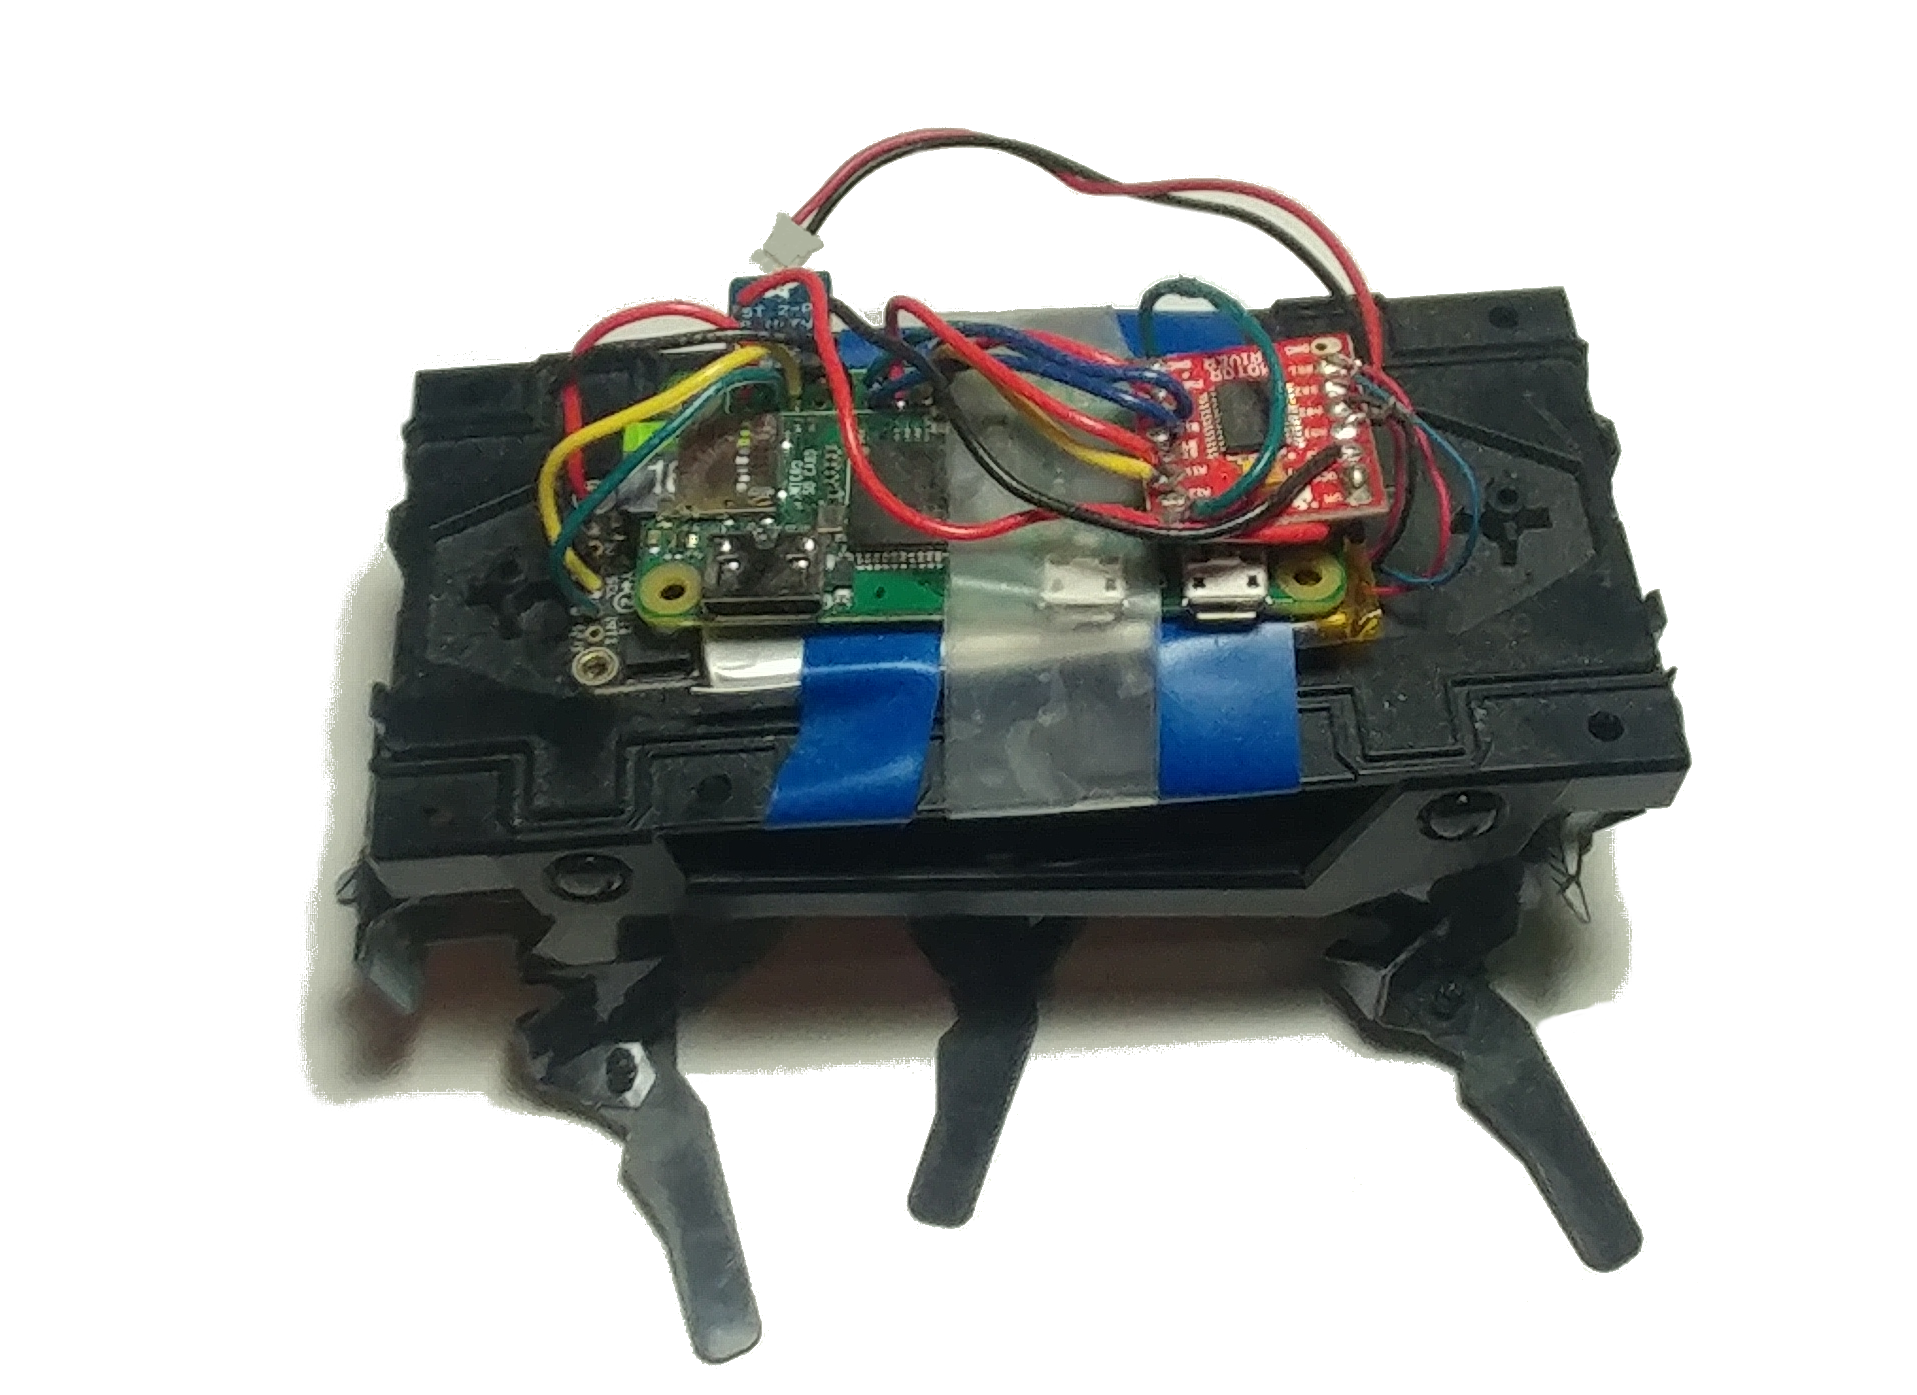
\includegraphics[width=\textwidth]{images/advert_edit.png}
    \caption{Assembeled Kamigami with Raspberry Pi 0 and attached peripherals}
    \label{fig:kamigami}
\end{figure}

\newpage

\tableofcontents
\newpage

\section{Introduction}
The \href{https://kamigamirobots.com/}{Kamigami toy} is an inexpensive platform for legged multi-robot research. With a fair bit of work, you can replace its circuit board with a Raspberry Pi 0 W, allowing you to use the robot in a ROS system, which allows for easier multirobot applications.

\section{Components} \label{components}

Here are the parts I used in my setup, but you can feel free to add or remove peripherals (like the IMU) as you see fit. I've hyperlinked product links, but you may find them cheaper from other sources.

\begin{itemize}
    \item \href{https://www.amzn.com/gp/product/B06ZYVMZC5/}{Kamigami toy}
    This is the actual robot you will be using. There are other models with different shells, but I believe the only differences are cosmetic, which will not be apparent for our uses since we will not build the Kamigami with the added shell pieces to reduce weight.
    
    \item \href{https://www.adafruit.com/product/3400}{Raspberry Pi 0 W}
    This model of the Raspberry Pi is gives us an inexpensive, light, and compact way to add a linux interface to the Kamigami. This Pi is equipped with Wifi and Bluetooth out of the box, making networking relatively painless.
    
    \item \href{https://www.sparkfun.com/products/14451}{Motor Driver}
    Sparkfun's motor driver board allows us to to control both speed and direction of both motors without much hassle. Although the output current is a bit low, I did not find this impeding the operation of my Kamigami.
    
    \item \href{https://www.adafruit.com/product/4480}{IMU} This cheap board comes with an accelerometer and gyroscope, but it may be worth spendign a bit extra to get something with a magnetometer for more accuracy. Still seems to do the job decently well.
    
    \item \href{https://www.amzn.com//dp/B07TDN2G18/}{SD Cards} These will be needed for storing the OS, ROS, and perhaps data log files for your robot.
    
    \item \href{https://www.adafruit.com/product/259}{LiPo Battery Charger} Depending on what battery you use to power the Kamigami, you will end up recharging it somewhat often. I have found this charger works relatively quickly and is pretty straightforward to use.
    
    \item \href{https://www.adafruit.com/product/1862}{JST-PH 2-Pin Right Angle Connector} Soldering this onto the Raspberry Pi makes it really easy to connect the battery for power and disconnect for charging.
    
    \item \href{https://www.adafruit.com/product/1862}{LiPo Battery} This battery was pretty satisfactory in terms of compromise between size, weight, cost, and power storage and can power the Kamigami robot with added peripherals for several hours of use before a recharge is needed.
    
\end{itemize}

\section{Setting up the Pi 0 W}

\textbf{Note: These instructions are incomplete. While I work on writing out the full instructions, please download and flash the disk image with everything pre-installed instead.}

You're welcome to flash an image of my OS with ROS setup, but I would recommend following the instructions below to get the most updated versions of everything, and to catch any mistakes/things I could be doing better. Note: there seem to be \href{https://github.com/alansrobotlab/rospberrypi}{instructions for getting ROS Melodic setup on the Pi 0}, but I have not followed these as I did not see them when I had started my project. In the future, I may attempt to migrate over to Melodic and will update the instructions here. My instructions are based off of \href{https://chenzhongxian.gitbooks.io/learning-robotics-using-ros/content/installing_ros_indigo_on_the_raspberry_pi.html}{this guide}.

\subsection{Installing Raspbian}

\begin{enumerate}
    \item First, you will want to \href{https://www.raspberrypi.org/downloads/raspberry-pi-os/}{get the newest version of Raspbian}, now called Raspberry Pi OS, flashed to your SD card. As of writing this, the newest version is based off of Debian Buster, so I will tailor my instructions to that. I would recommend the light/minimal version, if it is available.
    
    \item You need to setup ROS repositories for your system so we can install ROS things. Make sure to substitute 'buster' with the approriate OS in use.
    \begin{minted}[breaklines, frame=single]{bash}
sudo sh -c 'echo "deb http://packages.ros.org/ros/ubuntu buster main" > /etc/apt/sources.list.d/ros-latest.list'
wget https://raw.githubusercontent.com/ros/rosdistro/master/ros.key -O - | sudo apt-key add -
    \end{minted}
    
    Make sure to run update \& upgrade commands too.
    
    \begin{minted}[breaklines, frame=single]{bash}
sudo apt-get update
sudo apt-get upgrade
    \end{minted}
    
    \item You will also need bootstrap dependencies.
    \begin{minted}[breaklines, frame=single]{bash}
sudo apt-get install python-pip python-setuptools python-yaml python-distribute python-docutils python-dateutil python-six
sudo pip install rosdep rosinstall_generator wstool rosinstall
    \end{minted}
    
    \item The last thing dependency wise to do is to initialize rosdep.
    \begin{minted}[breaklines, frame=single]{bash}
sudo rosdep init
rosdep update
    \end{minted}
    
    \item Now it's time to move on to starting the actual build process. You will want to make some kind of directory to serve as the ROS workspace for your core ROS packages and go there.
    \begin{minted}[breaklines, frame=single]{bash}
mkdir ~/ros_ws
cd ~/ros_ws
    \end{minted}
    
    \item 
    
    
\end{enumerate}

\subsection{Installing ROS}

\subsection{Getting ROS Packages}

\section{Adding the Pi 0 W to the Kamigami}

\subsection{Removing Kamigami Electronics}

\subsection{Wiring}

Before mounting all add components to the kamigami, I would aA Fritzing diagram of the circuit is shown below; the Fritzing file should be in the same directory as this document.
The pinout for the Raspberry Pi can be seen \href{https://pinout.xyz}{here},
and the pinouts for other components can be viewed at the approriate pages in the \hyperref[components]{components section}.

\begin{figure}[H]
    \centering
    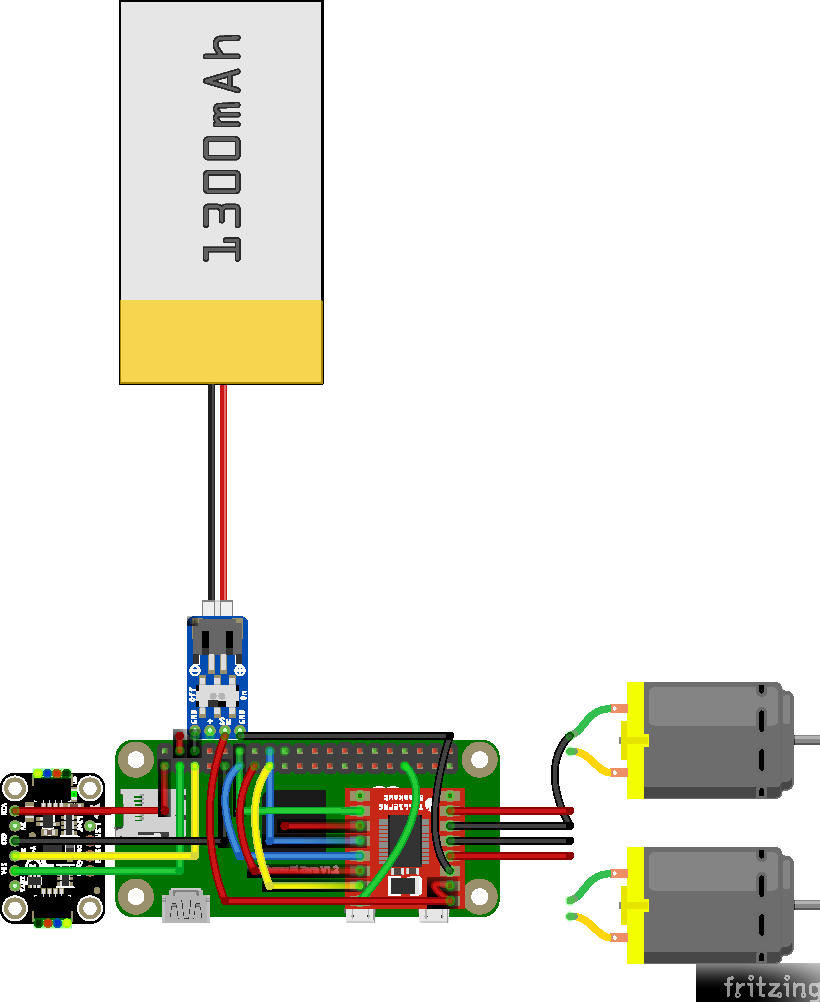
\includegraphics[width=.75\textwidth]{images/wiring.pdf}
    \caption{Wiring of Raspberry Pi 0}
    \label{fig:wiring}
\end{figure}

As we can see, every component is powered by a single LiPo battery. A 3.7V 1300 mAh battery is show in the image, but my implementation uses a 3.7V 1200 mAh battery. The Raspberry Pi and motor drivers recieve power directly from the battery, and the IMU is powered from the Raspberry Pi 0's 3.3V output. Notice that the Raspberry Pi is taking in 3.7V into its 5V power input; this is fine as the Raspberry Pi internally steps down the power to 3.3V for all pins. The DC motors in the image refer to motors on actual Kamigami, which you aren't expected to remove but you should wire into the motor driver.

\subsection{Mounting}
After completing the wiring, we can affix the components to the kamigami.


\section{Network Setup}

\subsection{Setup Hostnames and Master}

\subsection{Allow ROS Master Machine to Launch Nodes on the Pi 0 W}

\section{Development}

The kamigami ROS package stack can be found at the \href{https://github.com/BML-MultiRobot/kamigami_common}{kamigami\_common github repo}. Here, every node, topic, message type, launch file is documented.

\end{document}
